\appendix
\section{DCQCN stability analysis}
\label{sec:dcqcn_stability_analysis}

We linearize the system by denoting $\delta {R_C}(t) = {R_C}(t) - R_C^*$,
$\delta {R_C}(t) = {R_C}(t) - R_C^*$, $\delta p(t) = p(t) - p^*$, $\delta \alpha
(t) = \alpha (t) - \alpha^*$, and $A = \left( {\frac{1}{B} + \frac{1}{{TR_C^*}}}
\right)$.  We again use Taylor series to simplify the expressions of $a, b, c,
d, e$ to handle the exponential forms like $(1-p)^x$.  Due to lack of space,
here we only just show the linearized expression for $\frac{{d\delta {R_C}}}{{dt}}$:
\begin{equation}
\small
\begin{array}{l}
\frac{{d\delta {R_C}}}{{dt}} =  - \frac{1}{2}{(R_C^*)^2}{\alpha ^*}\delta p - \frac{1}{2}{p^*}R_C^*{\alpha ^*}\delta R_C \\
 - \frac{1}{2}{p^*}R_C^*{\alpha ^*}\delta {R_C} - \frac{1}{2}{p^*}{(R_C^*)^2}\delta \alpha \\
 + \frac{A}{2}\left( {R_C^*\delta {R_T} - R_C^*\delta {R_C} + R_T^*\delta {R_C} - R_C^*\delta R_C} \right)\\
 - \left( {\frac{1}{2} + \frac{A}{4}} \right)\left( {{p^*}R_C^*\delta {R_T} - {p^*}R_C^*\delta {R_C} + {p^*}R_T^*\delta {R_C}} \right)\\ 
 - \left( {\frac{1}{2} + \frac{A}{4}} \right)\left( {{p^*}R_C^*\delta R_C - R_C^*R_T^*\delta p + {{(R_C^*)}^2}\delta p} \right)
\end{array}
\end{equation}
Using Laplace transform, we get:
\begin{equation}
\small
\begin{array}{l}
s{R_C}(s) - \delta {R_C}(0) = \\
\left( { - \frac{1}{2}{{(R_C^*)}^2}{\alpha ^*} - \left( {\frac{1}{2} + \frac{A}{4}} \right)R_C^*R_T^* + \left( {\frac{1}{2} + \frac{A}{4}} \right){{(R_C^*)}^2}} \right){e^{ - s\tau *}}p(s)\\
 + \left( { - \frac{1}{2}{p^*}R_C^*{\alpha ^*} - \frac{A}{2}R_C^* + \left( {\frac{1}{2} + \frac{A}{4}} \right){p^*}R_C^*} \right){e^{ - s\tau *}}{R_C}(s)\\
 + \left( { - \frac{1}{2}{p^*}R_C^*{\alpha ^*} - \frac{A}{2}R_C^* + \frac{A}{2}R_T^* }\right){R_C}(s)\\
 + \left( { \left( {\frac{1}{2} + \frac{A}{4}} \right){p^*}R_C^* - \left( {\frac{1}{2} + \frac{A}{4}} \right){p^*}R_T^*} \right){R_C}(s)\\
 - \frac{1}{2}{p^*}{(R_C^*)^2}\alpha (s)\\
 + \left( {\frac{A}{2}R_C^* - \left( {\frac{1}{2} + \frac{A}{4}} \right){p^*}R_C^*} \right){R_T}(s)
\end{array}
\end{equation}
With Laplace transform of the other equations, we can use ${R_C}(s)$ to express
${R_T}(s)$, $p(s)$ and $\alpha (s)$.  We then derive the characteristic equation
of ${R_C}(s)$. Finally we compute the phase margin values of the characteristic equation
with different parameters.


\section{Proof of DCQCN convergence}
\label{sec:alpha_proof}

Below we provide the additional details of our proof. 
Figure~\ref{fig:dcqcn_convergence_detailed} illustrates some of the variables we use.

\para{Part I: The analysis of $R_T$.}
During the consecutive additive rate increase, {\em i.e.,} 
$\forall t \in ({T_k} + 1,{T_{k + 1}}]$, $R_C^{(i)}$ and $R_T^{(i)}$ 
have following relationship according to DCQCN's definition:
\begin{equation}
\small
R_C^{(i)}(t + 1) = \frac{1}{2}\left( {R_C^{(i)}(t) + R_T^{(i)}(t + 1)} \right)\\
\label{ref:discrete_rc}
\end{equation}
\begin{equation}
\small
R_T^{(i)}(t + 1) = R_T^{(i)}(t) + {R_{AI}}
\label{ref:discrete_rt}
\end{equation}
By (\ref{ref:discrete_rc})-$\frac{1}{2}\times$(\ref{ref:discrete_rt}), we get:
\begin{equation}
\small
\begin{array}{l}
R_C^{(i)}(T_{k + 1}) - R_T^{(i)}(T_{k + 1}) + {R_{AI}}\\
 = \frac{1}{2}\left( {R_C^{(i)}(T_{k + 1} - 1) - R_T^{(i)}(T_{k + 1} - 1) + {R_{AI}}} \right)\\
 = ... = {\left( {\frac{1}{2}} \right)^{\Delta {T_k}-1}}\left( {R_C^{(i)}({T_k} + 1) - R_T^{(i)}({T_k} + 1) + {R_{AI}}} \right)
\end{array}
\end{equation}
From this, we know that during a consecutive additive rate increase phase, $R_T^{(i)} - R_C^{(i)}$
will converge towards $R_{AI}$ exponentially. In addition, at the beginning of the phase, 
$R_C^{(i)}({T_k} + 1) = R_T^{(i)}({T_k})$ (Figure~\ref{fig:dcqcn_convergence}). Therefore:
%In common cases, the step of additive increase,
%$\Delta {T_k} - 1$, is around 10 or even more\footnote{This can be easily estimated by numerical approaches, 
%thus omitted for brevity}. 
%Also, due to DCQCN definition, we have $R_C^{(i)}({T_k} + 1) = R_T^{(i)}({T_k} + 1)$
%as shown in Figure~\ref{fig:dcqcn_convergence}. 
%Therefore, we can safely approximate $R_T^{(i)}$ by:
\begin{equation}
\small
R_T^{(i)}({T_k}) = R_C^{(i)}({T_k}) + \left( 1 - ({\frac{1}{2}})^{\Delta {T_k}-1}\right){R_{AI}},\forall k = 1,2,...
\label{eq:convergence_rt}
\end{equation}

\begin{figure}[t]
\center
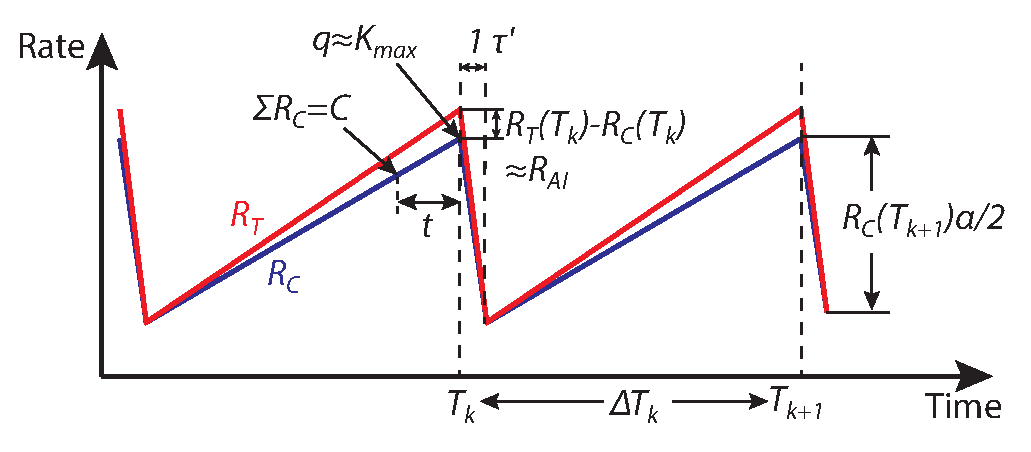
\includegraphics[width=0.4\textwidth]{figures/dcqcn_convergence.eps}
\caption{A more detailed view of DCQCN's AIMD-style updates of flow rate.}
\label{fig:dcqcn_convergence_detailed}
\end{figure}

\para{Part II: The lower bound of $\alpha$.}
To prove Equation~\ref{eq:converge_alphastar}, we first need to estimate $\Delta T_k$
using $\alpha$. In the period of $\Delta T_k$, after the first time unit of rate
decrease, the aggregated flow rates will climb back to $R_T(T_{k+1})$ by
$NR_{AI}$ every time unit.  Thus we have:
\begin{equation}
\small\Delta {T_k} = 1 + \frac{{\sum\limits_{i = 1}^N {\left( {R_T^{(i)}({T_{k + 1}}) - \left( {1 - {\alpha ^{(i)}}({T_k})/2} \right)R_C^{(i)}({T_k})} \right)} }}{{N{R_{AI}}}}
\end{equation}
Suppose $\alpha^{(i)}({T_k})$ already converged to the same value $\alpha ({T_k})$, as guaranteed by
Equation~\ref{eq:converge_alphaarray}. We simplify it as:
\begin{equation}
\small
\begin{array}{l}
\Delta {T_k} = 1 + \frac{{\sum\limits_{i = 1}^N {R_T^{(i)}({T_{k + 1}})}  - \left( {1 - \alpha ({T_k})/2} \right)\sum\limits_{i = 1}^N {R_C^{(i)}({T_k})} }}{{N{R_{AI}}}}\\
 \approx 1 + \frac{{\left( {C + tN{R_{AI}} + N{R_{AI}}} \right) - \left( {1 - \alpha ({T_k})/2} \right)\left( {C + tN{R_{AI}}} \right)}}{{N{R_{AI}}}}\\
 = 2 + \left( {\frac{t}{2} + \frac{C}{{2N{R_{AI}}}}} \right)\alpha ({T_k})
\end{array}
\label{eq:converge_tk}
\end{equation}
Where $t$ is the time it takes for the flows to build up queue and get packets ECN-marked, after
the aggregated flow rates exceed link capacity $C$, as shown in Figure~\ref{fig:dcqcn_convergence}.
We can estimate $t$ by the queue being built up:
\begin{equation}
\small
\begin{array}{l}
N\tau '\left( {{R_{AI}} + 2{R_{AI}} + ... + t{R_{AI}}} \right) = {Q_{ECN}} \le {K_{\max }}\\
 \Rightarrow t \le \left( { - 1 + \sqrt {1 + \frac{{8{K_{\max }}}}{{N{R_{AI}}\tau '}}} } \right)/2
\end{array}
\end{equation}
Now, we prove Equation~\ref{eq:converge_alphastar}, where $\alpha^*$ is the solution of the following:
\begin{equation}
\small
{\alpha ^*} = {(1 - g)^{\Delta {T^*}}}\left( {(1 - g){\alpha ^*} + g} \right)
\end{equation}
Once Equation~\ref{eq:converge_alphastar} is proved, $\alpha ({T_k})$ has a non-zero lower bound, 
$R_C$ will converge exponentially.
We prove this by mathematical induction. The initial value of $\alpha$ is 1, as defined
by DCQCN. So, $\alpha ({T_0}) > {\alpha ^*} > 0$. Now assuming $\alpha ({T_k}) > {\alpha ^*} > 0$, we 
prove $\alpha ({T_k}) > \alpha ({T_{k+1}}) > {\alpha ^*}$. We define $f(\alpha)$ as the RHS of 
Equation~\ref{eq:converge_alpha}:
\begin{equation}
\small
f(\alpha ) = {(1 - g)^{2 + \left( {\frac{t}{2} + \frac{C}{{2N{R_{AI}}}}} \right)\alpha }}\left( {(1 - g)\alpha  + g} \right)
\end{equation}
By analyzing the derivative of $f(\alpha )$, it is not hard to see that with common parameter 
settings, $f(\alpha )$ is monotonically increasing. Therefore, 
\begin{equation}
\small
\alpha ({T_{k + 1}}) = f\left( {\alpha ({T_k})} \right) > f\left( {{\alpha ^*}} \right) = {\alpha ^*}
\label{eq:appendix_left}
\end{equation}
In addition, because $\alpha ({T_k}) > {\alpha ^*} => \Delta {T_k} > \Delta {T^*}$, 
$\alpha^{*}$ satisfies:
\begin{equation}
\small
{\alpha ^*} > {(1 - g)^{\Delta {T_k}}}\left( {(1 - g){\alpha ^*} + g} \right)
\end{equation}
Subtract this from Equation~\ref{eq:converge_alpha}, we see $\alpha ({T_k})$ is exponentially 
converging towards $\alpha ^*$:
\begin{equation}
\small
\alpha ({T_{k + 1}}) - {\alpha ^*} < {(1 - g)^{\Delta {T_n}}}\left( {\alpha ({T_k}) - {\alpha ^*}} \right)
\label{eq:appendix_right}
\end{equation}
Equation~\ref{eq:appendix_left} and~\ref{eq:appendix_right} lead to 
${\alpha ^*} < \alpha ({T_{k + 1}}) < \alpha ({T_k})$. $\qed$
